\documentclass{article}

\PassOptionsToPackage{numbers,compress}{natbib}
\usepackage{neurips_2026}

\usepackage[utf8]{inputenc}
\usepackage[T1]{fontenc}
\usepackage{hyperref}
\usepackage{url}
\usepackage{booktabs}
\usepackage{amsfonts}
\usepackage{amsmath}
\usepackage{amssymb}
\usepackage{microtype}
\usepackage{xcolor}
\usepackage{graphicx}
\graphicspath{{figures/}}

\title{Routing Visual Evidence Under Domain Shift: Three-Way Factorization for Cross-Domain Audio-Visual Deepfake Detection}

\author{%
  Zhili Nicholas Liang \\
  University of Melbourne \\
  Melbourne, Victoria, Australia \\
  \texttt{nnliang@student.unimelb.edu.au} \\
  \And
  Soyeon Caren Han \\
  University of Melbourne \\
  Melbourne, Victoria, Australia \\
  \texttt{caren.han@unimelb.edu.au} \\
  \And
  Qizhou Wang \\
  University of Melbourne \\
  Melbourne, Victoria, Australia \\
  \texttt{mike.wang@unimelb.edu.au} \\
  \And
  Christopher Leckie \\
  University of Melbourne \\
  Melbourne, Victoria, Australia \\
  \texttt{caleckie@unimelb.edu.au} \\
}

\newcommand{\method}{\textsc{TriRoute}}
\newcommand{\R}{\mathbb{R}}

\begin{document}

\maketitle

\begin{abstract}
Source-trained audio-visual deepfake detectors fail under dataset shift by routing decisions through domain-correlated shortcuts rather than transferable manipulation evidence. We propose \method, a factorized detector that decomposes frozen AV-HuBERT features into shared cross-modal content, modality-unique manipulation cues, and a residual branch that absorbs domain-sensitive nuisance. A domain push-pull objective attracts shortcut information into the residual branch while discouraging easy domain prediction from the task branch, which reads only the shared and unique factors. On the AV-Deepfake1M$\rightarrow$FakeAVCeleb cross-domain benchmark, \method\ improves FakeVideo-RealAudio (FV-RA) AUC from $0.523$ to $0.659$ using only source-domain pseudo-labels and further to $0.677$ under standard UDA, while adding domain adversarial pressure to a two-way representation degrades FV-RA to $0.441$. The small gap between label settings ($+0.018$) demonstrates that representation structure matters more than domain-label fidelity. Head ablations confirm that masking $u_v$ drops FV-RA by $0.354$; input masking shows full audio masking improves \method's FV-RA ($+0.039$) while full visual masking causes a $3.4\times$ larger drop than the two-way baseline. These results establish a change in evidence routing as the primary driver of cross-domain gain.
\end{abstract}

\section{Introduction}

Audio-visual deepfakes have become harder to detect as modern generators jointly manipulate lip motion, facial appearance, and speech with high realism. Supervised detectors trained on a single dataset frequently fail at test time by overfitting to generator fingerprints, compression artifacts, or annotation shortcuts rather than transferable manipulation evidence. This problem is especially acute under dataset shift, where the easiest predictive signal is often not the manipulation itself, but a domain-correlated shortcut.

Prior work on audio-visual synchronization, speech-aware representations, and joint modeling of shared and modality-specific evidence has improved robustness by anchoring detection to cross-modal consistency \citep{feng2023avad, liang2024speechforensics, smeu2025avhalign, du2025cad}. However, these methods do not resolve cross-domain audio-visual forensics, where the representation must separate three qualitatively different signals: speech content, visual manipulation evidence, and domain-correlated nuisance. When these factors remain entangled, a detector may contain useful visual evidence and still ignore it because source-domain shortcuts offer an easier optimization path.

We frame cross-domain audio-visual deepfake detection as an evidence-routing problem and propose \method, a three-way factorized detector. \method\ decomposes frozen AV-HuBERT features into a shared cross-modal content branch, modality-unique manipulation cues, and a domain-residual branch explicitly trained to absorb dataset-level nuisance. The prediction head reads only the shared and unique factors. Our core contribution is structural separation that changes which evidence the detector uses under shift---not a claim of global domain invariance.

\paragraph{Contributions.} Our contributions are summarised as follows:
\begin{enumerate}
\item \textbf{Three-Way Factorized Architecture}: We propose \method, which separates a dedicated domain-residual branch as an explicit shortcut sink and restricts the prediction head to shared content and modality-unique manipulation factors, assigning each signal type a separate structural role.
\item \textbf{Structural Separation as the Primary Gain Driver}: Adding GRL to a two-way representation degrades FV-RA AUC from $0.523$ to $0.441$; \method\ improves it to $0.659$ (no-target-data) and $0.677$ (UDA); three-way factorization without domain supervision already reaches $0.626$. The small gap between label settings ($+0.018$) confirms that representation structure matters more than domain-label fidelity.
\item \textbf{Routing-Focused Cross-Domain Benchmark}: We establish an AV1M$\rightarrow$FAVC cross-domain evaluation centered on FV-RA---the category where audio shortcuts are deliberately unhelpful and the detector must use visual evidence. Subspace probes, head ablations, and input perturbations collectively support a routing-based explanation.
\end{enumerate}

\section{Related Work}

\paragraph{Audio-visual deepfake detection.}
Multimodal deepfake detection exploits the constraint that authentic speech, lip motion, and facial dynamics must remain mutually consistent over time. Methods range from direct fusion and synchronization cues \citep{zhou2021jointav, chung2016syncnet} to self-supervised anomaly detection and explicit modality-shared/specific decompositions \citep{feng2023avad, liang2024speechforensics, smeu2025avhalign, du2025cad}. These approaches improve over purely artifact-based detectors but optimize a single prediction pathway, leaving the question of which subspace drives decisions under shift unaddressed.

\paragraph{Evaluation protocols.}
Most audio-visual deepfake work reports in-dataset splits. The closest published cross-domain bridge is AVH-Align \citep{smeu2025avhalign}, which reports supervised AV1M$\rightarrow$FAVC scores while diagnosing leading-silence shortcuts. Our contribution is an AV1M$\rightarrow$FAVC stress test with modality-category reporting and routing analyses specifically focused on FV-RA.

\paragraph{Speech-aware multimodal representations.}
AV-HuBERT \citep{shi2022avhubert} captures both local synchronization and longer-term speech structure, proving useful for forensic analysis and synchronization-based detection \citep{liang2024speechforensics, smeu2025avhalign}. \method\ uses the same backbone but adds an explicit factorization layer so the downstream detector discards nuisance factors rather than letting them leak into the prediction head.

\paragraph{Domain-adversarial learning.}
Domain-adversarial training \citep{ganin2016dann} applies a gradient-reversal classifier to discourage domain-predictive encoding. On an undifferentiated representation this pressure is diffuse and can destabilize genuinely predictive signals. \method\ addresses this by separating a dedicated residual branch whose sole role is to absorb domain-correlated signal and pairing it with a forward domain-prediction objective that pulls domain information into the residual. The adversarial pressure then acts only on the task branch, making the push-pull effect targeted rather than global.

\section{Problem Setting}

We study cross-dataset audio-visual deepfake detection. Training samples $\mathcal{D} = \{(x_i^v, x_i^a, y_i, d_i)\}_{i=1}^N$ include a visual sequence $x_i^v$, synchronized audio $x_i^a$, label $y_i \in \{0,1\}$, and domain indicator $d_i \in \{1,\dots,M\}$. Task supervision uses AV-Deepfake1M clips. Domain supervision is provided in two settings: (i)~\emph{no-target-data}, using speaker-group pseudo-labels derived from AV1M ($d = \mathrm{hash}(\mathrm{speaker\_id})\bmod 2$) with no FakeAVCeleb data at any training stage; and (ii)~\emph{UDA}, additionally using unlabelled real-only FakeAVCeleb clips as domain identity, with no manipulation labels. Test labels are never observed during training.

Our goal is a scoring function $f(x^v, x^a)$ that remains predictive under domain shift by isolating manipulation evidence from non-transferable domain signals. We test the claim that factorization changes representation usage and routing under shift; we do not require the task branch to become fully domain-invariant.

\section{Method}

\subsection{Overview}

Figure~\ref{fig:overview} shows \method's architecture. Starting from frozen AV-HuBERT features $z_v, z_a \in \R^{1024}$, we first extract shared cross-modal factors and modality-specific hidden states:
\begin{equation}
\big[s_v, h_v\big] = F_v(z_v), \qquad \big[s_a, h_a\big] = F_a(z_a),
\end{equation}
where $s_v, s_a$ are shared task-relevant factors and $h_v, h_a$ contain the remaining modality-specific signal. We split the modality-specific states into unique task-relevant and residual components:
\begin{equation}
\big[u_v, r_v\big] = G_v(h_v), \qquad \big[u_a, r_a\big] = G_a(h_a).
\end{equation}
The task and residual representations are:
\begin{equation}
Z_{\mathrm{task}} = \mathrm{cat}(s_v, u_v, s_a, u_a), \qquad
Z_{\mathrm{res}} = \mathrm{cat}(r_v, r_a).
\end{equation}
The prediction head reads only $Z_{\mathrm{task}}$. The residual branch $Z_{\mathrm{res}}$ is supervised to absorb domain-correlated signal and is excluded from all detection paths. We refer to $s_v, s_a$ as \emph{content} factors, $u_v, u_a$ as \emph{manipulation} factors, and $r_v, r_a$ as \emph{domain} factors throughout.

\subsection{Three-Way Factorization}

\paragraph{Manipulation factor.}
The modality-unique components $u_v$ and $u_a$ encode evidence that cannot be explained by authentic cross-modal correspondence. The visual-unique component $u_v$ is the primary carrier for FV-RA; $u_a$ supports audio-fake cases. These unique components feed the task head together with the shared content factors.

\paragraph{Content factor.}
Shared factors capture speech semantics and identity-preserving motion that should generalise across domains. We align them across modalities with:
\begin{equation}
\mathcal{L}_{\mathrm{align}} = - \sum_{t=1}^T
\log
\frac{\exp(\mathrm{sim}(s_{v,t}, s_{a,t})/\tau)}
{\sum_{j \in \mathcal{N}(t)} \exp(\mathrm{sim}(s_{v,t}, s_{a,j})/\tau)},
\end{equation}
where $\mathrm{sim}(\cdot,\cdot)$ is cosine similarity, $\tau$ is a temperature, and $\mathcal{N}(t)$ is a local temporal window.

\paragraph{Domain factor.}
The residual branch is optimized to predict source domain:
\begin{equation}
\mathcal{L}_{\mathrm{dom}} = \mathrm{CE}(C_d(Z_{\mathrm{res}}), d),
\end{equation}
making $Z_{\mathrm{res}}$ an information sink for codec, resolution, and dataset-construction artifacts.

\subsection{Detection and Domain Push-Pull Objectives}

We predict clip-level fake probability from $Z_{\mathrm{task}}$:
\begin{equation}
\hat{y} = C_y(Z_{\mathrm{task}}), \qquad \mathcal{L}_{\mathrm{fake}} = \mathrm{BCE}(\hat{y}, y).
\end{equation}
Task and residual factors are separated by an orthogonality penalty:
\begin{equation}
\mathcal{L}_{\mathrm{ortho}} =
\left\| s_v^\top r_v \right\|_F^2
+ \left\| s_a^\top r_a \right\|_F^2
+ \left\| u_v^\top r_v \right\|_F^2
+ \left\| u_a^\top r_a \right\|_F^2.
\end{equation}
A gradient-reversal domain classifier suppresses easy domain prediction from the task branch:
\begin{equation}
\mathcal{L}_{\mathrm{adv}} =
\mathrm{CE}(C_{\mathrm{adv}}(\mathrm{GRL}(Z_{\mathrm{task}})), d).
\end{equation}
The full objective combines all terms:
\begin{equation}
\mathcal{L}
=
\mathcal{L}_{\mathrm{fake}}
+
\lambda_{\mathrm{align}} \mathcal{L}_{\mathrm{align}}
+
\lambda_{\mathrm{dom}} \mathcal{L}_{\mathrm{dom}}
+
\lambda_{\mathrm{adv}} \mathcal{L}_{\mathrm{adv}}
+
\lambda_{\mathrm{ortho}} \mathcal{L}_{\mathrm{ortho}}.
\end{equation}

\begin{figure}[t]
    \centering
    
\includegraphics[width=0.97\linewidth]{overview.pdf}
    \caption{Conceptual overview of \method. Frozen AV-HuBERT features are decomposed into shared cross-modal factors $(s_v,s_a)$, modality-unique factors $(u_v,u_a)$, and residual factors $(r_v,r_a)$. The task head reads only the shared and unique factors; domain push-pull concentrates nuisance in $Z_{\mathrm{res}}$ and discourages easy domain prediction from $Z_{\mathrm{task}}$.}
    \label{fig:overview}
\end{figure}

\section{Experiments}

\subsection{Datasets and Evaluation}

We train on AV-Deepfake1M (AV1M) \citep{cai2024avdeepfake1m} and evaluate on the FakeAVCeleb (FAVC) \citep{khalid2021fakeavceleb} 70/30 public test split ($N=6{,}667$), following the evaluation protocol of \citet{smeu2025avhalign}. We additionally report directional results on AVLips \citep{como2024lips}. Performance is reported as threshold-free AUC and average precision (AP) for three categories: RealVideo-FakeAudio (RV-FA), FakeVideo-RealAudio (FV-RA), and FakeVideo-FakeAudio (FV-FA). FV-RA is the most diagnostic category: audio shortcuts are unhelpful there, forcing the model to rely on visual manipulation evidence. All results report means over three random seeds unless otherwise stated.

\subsection{Baselines}

We compare against AVH-Align/sup \citep{smeu2025avhalign}---the only published method training on AV1M and evaluating on FAVC under a compatible AV-HuBERT protocol---and a progression of internal ablation baselines. The \textbf{two-way baseline} applies coarser two-branch factorization without domain routing. The \textbf{two-way + domain-adversarial control} adds GRL to the two-way representation without three-way factorization, isolating the effect of domain pressure alone. The \textbf{three-way factorization without domain push-pull} applies the same structural decomposition as \method\ but omits both the domain-prediction and adversarial objectives. All variants use identical AV-HuBERT features and the same classifier backbone.

\subsection{Implementation Details}

\method\ uses frozen AV-HuBERT \citep{shi2022avhubert} features ($C=1{,}024$, 25\,fps, mouth-crop visual stream). Factorization modules and classifier are lightweight MLPs (three to four layers, LayerNorm, ReLU) with 256-dimensional shared, unique, and residual components per modality. Training uses Adam with learning rate $10^{-3}$, batch size 1 (variable-length clips), and patience-20 early stopping on validation AUC over up to 100 epochs. We fix $\lambda_{\mathrm{align}} = 0.5$, $\lambda_{\mathrm{dom}} = 1.0$, $\lambda_{\mathrm{adv}} = 1.0$, $\lambda_{\mathrm{ortho}} = 0.1$, and GRL $\alpha = 1.0$.

\section{Results and Analysis}

\subsection{Cross-Domain Detection Performance}

Table~\ref{tab:main} compares \method\ against AVH-Align/sup and internal ablations. The two-way baseline achieves near-ceiling performance on RV-FA and FV-FA but barely exceeds chance on FV-RA ($0.523$ AUC). Adding domain adversarial pressure to the two-way representation degrades FV-RA to $0.441$, confirming that domain pressure alone is insufficient and destabilizes the model's audio-dominant routing. Three-way factorization without domain push-pull raises FV-RA to $0.626/0.973$. \method\ with pseudo-domain labels achieves $0.659/0.974$ FV-RA; the UDA variant reaches $0.677/0.976$. The small increment ($+0.018$) demonstrates that representation structure matters more than domain-label fidelity. The gain concentrates in FV-RA, confirming it as the intended visual-routing stress test. Figure~\ref{fig:seed_variance} shows all individual seed results, confirming the gain is consistent and not driven by a single outlier.

\begin{table}[t]
    \centering
    \caption{Cross-domain detection on FakeAVCeleb (AV1M $\to$ FAVC, $N=6{,}667$). Each numeric cell reports mean AUC/AP; ablation rows are means over three seeds (43--45). The AVH-Align/sup row is the single AV1M-trained checkpoint from \citet{smeu2025avhalign}. RV-FA~=~RealVideo-FakeAudio; FV-RA~=~FakeVideo-RealAudio; FV-FA~=~FakeVideo-FakeAudio. \emph{No target data}: \method\ uses AV1M speaker-group pseudo-domain labels only; no FakeAVCeleb data enters training. \emph{+UDA}: additionally uses unlabelled real-only FakeAVCeleb clips as domain identity; no manipulation labels from FakeAVCeleb are used.}
    \label{tab:main}
    \resizebox{\linewidth}{!}{%
    \begin{tabular}{llcccc}
        \toprule
        Method & Structure & Overall & RV-FA & FV-RA & FV-FA \\
        \midrule
        AVH-Align/sup \citep{smeu2025avhalign} & two-way supervised & $0.777/0.994$ & $0.999/0.999$ & $0.519/0.955$ & $0.999/1.000$ \\
        \midrule
        Two-way baseline & two-way factorization & $0.779/0.994$ & $1.000/1.000$ & $0.523/0.957$ & $0.999/1.000$ \\
        Two-way + domain-adversarial control & two-way + GRL & $0.741/0.993$ & $1.000/1.000$ & $0.441/0.949$ & $0.998/1.000$ \\
        Three-way, no domain push-pull & three-way factorization & $0.827/0.996$ & $1.000/1.000$ & $0.626/0.973$ & $0.999/1.000$ \\
        \method, no target data (ours) & three-way + push-pull & $0.841/0.996$ & $1.000/1.000$ & $0.659/0.974$ & $0.997/1.000$ \\
        \method\ + UDA (ours) & three-way + push-pull + UDA & $\mathbf{0.850/0.996}$ & $1.000/1.000$ & $\mathbf{0.677/0.976}$ & $0.997/1.000$ \\
        \bottomrule
    \end{tabular}}
\end{table}

\begin{figure}[t]
    \centering
    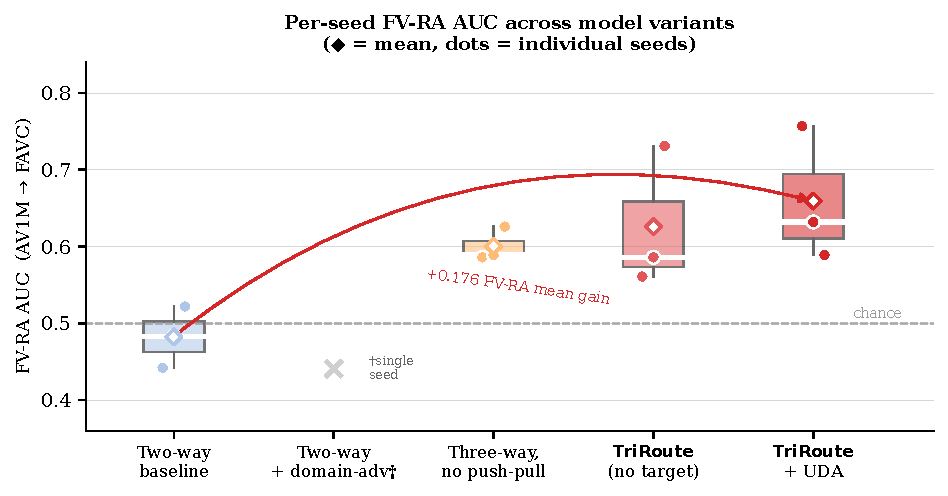
\includegraphics[width=0.72\linewidth]{seed_variance.pdf}
    \caption{Per-seed FV-RA AUC for each model variant. Boxes show the interquartile range; the diamond marks the mean; individual dots show each seed. All three \method\ seeds exceed all three two-way baseline seeds, and the mean gain is not driven by a single outlier.}
    \label{fig:seed_variance}
\end{figure}

\paragraph{Reverse-direction generalisation (FAVC $\to$ AV1M).}
To verify the routing benefit is not specific to the AV1M$\to$FAVC direction, we train each variant on FakeAVCeleb and evaluate on AV-Deepfake1M validation ($N=2{,}000$). Table~\ref{tab:reverse} reports overall AUC/AP as mean$\,\pm\,$std over four seeds (42--45) for no-target-data variants and three seeds (42--44) for UDA. The only published FAVC-trained baseline with an available checkpoint is AVH-Align/sup \citep{smeu2025avhalign} (AUC~$0.677$). \method\ in the no-target-data setting attains the best overall AUC ($0.729$), improving over AVH-Align/sup by $+0.052$, over the two-way baseline by $+0.059$, and over the three-way no-push-pull variant by $+0.047$.

\begin{table}[t]
    \centering
    \caption{Reverse-direction cross-domain detection (FAVC $\to$ AV1M val, $N=2{,}000$). Mean$\,\pm\,$std over four seeds (42--45), except \method\,+UDA (three seeds, 42--44). The AVH-Align/sup row is the single official FAVC-trained checkpoint from \citet{smeu2025avhalign}; no std reported. The two-way + GRL row is omitted as it was not included in the reverse-direction sweep.}
    \label{tab:reverse}
    \small
    \begin{tabular}{llcc}
        \toprule
        Method & Structure & Overall AUC & Overall AP \\
        \midrule
        AVH-Align/sup \citep{smeu2025avhalign} & supervised baseline & $0.677$ & $0.813$ \\
        \midrule
        Two-way baseline                 & two-way factorization        & $0.670 \pm 0.032$ & $0.812 \pm 0.014$ \\
        Three-way, no domain push-pull   & three-way factorization      & $0.682 \pm 0.048$ & $0.819 \pm 0.033$ \\
        \method, no target data (ours)   & three-way + push-pull        & $\mathbf{0.729 \pm 0.078}$ & $\mathbf{0.852 \pm 0.052}$ \\
        \method\ + UDA (ours)            & three-way + push-pull + UDA  & $0.689 \pm 0.051$ & $0.813 \pm 0.017$ \\
        \bottomrule
    \end{tabular}
\end{table}

\subsection{Subspace Evidence: Routing Without Full Invariance}

Table~\ref{tab:probe} summarizes probe results for key visual subspaces. The visual-unique factor of \method\ is the strongest OOD carrier, reaching AUC of $0.924$ on AV1M$\rightarrow$FAVC---substantially above the two-way task branch ($0.705$) and all other subspaces. All subspaces remain highly domain-predictive (AUC $>0.96$), confirming that the cross-domain gain reflects a change in evidence routing rather than full domain invariance. Figure~\ref{fig:analysis} (left) displays these numbers alongside domain-probe AUCs.

\begin{table}[t]
    \centering
    \caption{Representative probe AUCs for key visual subspaces. The OOD probe trains on AV1M and evaluates on the FAVC test split; the domain probe measures dataset predictability. The visual-unique factor of \method\ is the strongest OOD carrier while remaining strongly domain-predictive.}
    \label{tab:probe}
    \small
    \begin{tabular}{lccc}
        \toprule
        Subspace & Dim. & OOD probe & Domain probe \\
        \midrule
        Two-way task branch $Z_c$ & 1024 & $0.705$ & $0.998$ \\
        Two-way visual factor $v_c$ & 512 & $0.891$ & $0.994$ \\
        Three-way shared visual $s_v$ & 256 & $0.814$ & $0.992$ \\
        Three-way unique visual $u_v$ & 256 & $0.825$ & $0.967$ \\
        \method\ shared visual $s_v$ & 256 & $0.726$ & $0.989$ \\
        \method\ unique visual $u_v$ & 256 & $\mathbf{0.924}$ & $0.976$ \\
        \bottomrule
    \end{tabular}
\end{table}

\subsection{Routing Evidence: Head Ablation}

Table~\ref{tab:ablation} quantifies how strongly each model's FV-RA performance depends on its visual branches, also visualised in Figure~\ref{fig:analysis} (right). For the two-way baseline, zeroing the visual task branch causes a negligible $-0.034$ drop, confirming the trained detector barely uses visual evidence for FV-RA. Three-way factorization without domain push-pull shows an intermediate drop ($-0.113$). For \method, masking the visual-unique manipulation factor alone causes a $-0.354$ drop, demonstrating that FV-RA decisions route primarily through $u_v$. The asymmetry is further confirmed by the audio direction: masking the two-way baseline's audio branch drops in-domain AUC from $0.997$ to $0.528$, confirming audio dominance rather than visual capacity failure in the baseline.

Figure~\ref{fig:routing} provides qualitative evidence. For the fake clip, $\|u_v^t\|$ peaks sharply in the manipulated lip region while the residual $\|r_v^t\|$ remains elevated throughout; for the real clip, both channels stay low and uniform.

\begin{table}[t]
    \centering
    \caption{Head-ablation analysis on FV-RA AUC. Each row zeros out one branch of the trained model and measures the FV-RA drop ($\Delta$FV-RA). Larger drop indicates heavier routing dependence on that branch. Bold shows the largest drop.}
    \label{tab:ablation}
    \resizebox{\linewidth}{!}{%
    \begin{tabular}{llccc}
        \toprule
        Model & Ablation & Baseline FV-RA & Ablated FV-RA & $\Delta$FV-RA \\
        \midrule
        Two-way baseline & mask visual task branch & $0.495$ & $0.461$ & $-0.034$ \\
        Three-way, no domain push-pull & mask visual branches & $0.586$ & $0.473$ & $-0.113$ \\
        \method & mask manipulation ($u_v$) & $0.721$ & $0.366$ & $\mathbf{-0.354}$ \\
        \bottomrule
    \end{tabular}}
\end{table}

\begin{figure}[t]
    \centering
    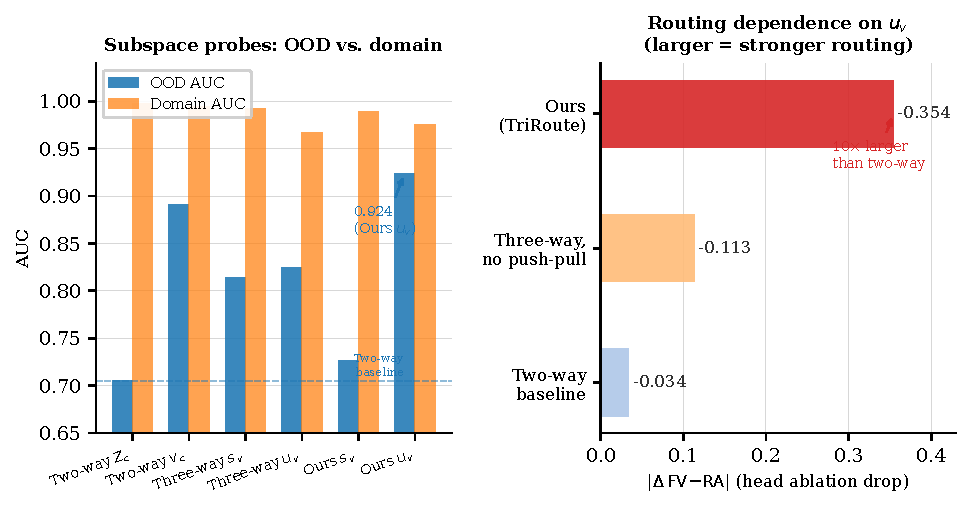
\includegraphics[width=0.97\linewidth]{analysis.pdf}
    \caption{\textbf{Left}: OOD probe AUC and domain-probe AUC for each visual subspace. \method's visual-unique channel ($u_v$, rightmost pair) achieves the highest OOD AUC ($0.924$) while remaining strongly domain-predictive ($0.976$), supporting a routing rather than invariance explanation. \textbf{Right}: Head-ablation routing sensitivity ($|\Delta\text{FV-RA}|$ when the visual branch is masked). \method's FV-RA decision is $10\times$ more dependent on the visual-unique manipulation factor than the two-way baseline.}
    \label{fig:analysis}
\end{figure}

\begin{figure}[t]
    \centering
    
\includegraphics[width=0.97\linewidth]{routing_map.pdf}
    \caption{Per-frame routing activation for a representative fake clip (top) and real clip (bottom). Visual-unique activations ($u_v$, blue) peak in the manipulated region of the fake clip; residual activations ($r_v$, orange) absorb the domain baseline throughout. Both channels remain low and uniform for the real clip, consistent with the head-ablation finding that FV-RA decisions route through $u_v$.}
    \label{fig:routing}
\end{figure}

\subsection{Input-Level Routing Verification}

As a model-agnostic complement to head ablation, we perturb input features on the FV-RA category and measure AUC change. If the trained head routes FV-RA decisions through the visual channel, full visual masking should cause a large drop; full audio masking should be neutral or beneficial, since FV-RA clips have real audio that may be a misleading signal. Table~\ref{tab:perturbation} reports mean FV-RA AUC over three seeds at full masking. Two patterns stand out. First, the two-way baseline barely changes under either masking ($\Delta_{\mathrm{audio}}=-0.021$, $\Delta_{\mathrm{visual}}=-0.077$), consistent with a model near chance on FV-RA. Second, \method\ shows a strongly asymmetric profile: full audio masking \emph{improves} FV-RA ($+0.039$) while full visual masking causes a $-0.265$ drop---a $3.4\times$ larger visual sensitivity than the two-way baseline. The improvement under audio masking confirms that \method\ actively suppresses a misleading real-audio signal when visual routing is established. Three-way factorization without push-pull shows an intermediate profile, matching its intermediate FV-RA AUC in Table~\ref{tab:main}.

\begin{table}[t]
    \centering
    \caption{FV-RA AUC under full input masking on the FakeAVCeleb FV-RA category. Each row reports mean over three seeds. Positive $\Delta_{\mathrm{audio}}$ indicates that removing the audio signal \emph{helps} FV-RA detection, confirming the model exploits the visual channel and suppresses misleading real-audio signal. Bold indicates best performance.}
    \label{tab:perturbation}
    \small
    \begin{tabular}{lcccc}
        \toprule
        Model & Baseline & $\Delta_{\mathrm{audio}}$ (full) & $\Delta_{\mathrm{visual}}$ (full) & Relative visual sensitivity \\
        \midrule
        Two-way baseline        & $0.546$ & $-0.021$ & $-0.077$ & $1.0\times$ \\
        Three-way, no push-pull & $0.616$ & $+0.040$ & $-0.137$ & $1.8\times$ \\
        \method\ (ours)         & $\mathbf{0.757}$ & $\mathbf{+0.039}$ & $\mathbf{-0.265}$ & $\mathbf{3.4\times}$ \\
        \bottomrule
    \end{tabular}
\end{table}

\subsection{Corrected Artifact Control}

A potential confound in AV1M-trained models is leading silence: fabricated clips sometimes begin with audio-free frames absent in authentic samples. We evaluate on leading-silence-trimmed preprocessed inputs (raw-waveform leading silence removed prior to AV-HuBERT extraction). FV-RA performance remains essentially stable: three-way without domain push-pull changes from $0.626$ to $0.624$; \method\ no-target-data changes from $0.731$ to $0.738$. The visual-fake gain is not driven by a leading-silence artifact.

\subsection{Domain Label Quality}
\label{sec:domain_label_quality}

The speaker-group pseudo-label is an extremely coarse proxy for the true AV1M-to-FAVC domain gap, partitioning training clips by speaker identity rather than encoding codec or acquisition differences. Despite this, it yields a $+0.136$ FV-RA gain over the two-way baseline ($0.523 \to 0.659$). Providing more accurate domain contrast via the UDA setting contributes a further modest gain ($0.659 \to 0.677$, $+0.018$). Domain supervision is helpful but secondary to the structural representation split.

\subsection{Comparison in AVH-Align Protocol}

Table~\ref{tab:avhalign_comparison} replicates the structure of Table~2 in \citet{smeu2025avhalign}, reporting AUC and AP on FakeAVCeleb and AV-Deepfake1M validation ($N=2{,}000$), with and without leading-silence trimming. After trimming, \method\ remains clearly stronger than the supervised AV1M-trained AVH-Align baseline on FAVC ($84.3$ vs.\ $70.8$ AUC), while trailing the strongest unsupervised VoxCeleb2-pretrained methods. This remaining gap reflects residual shortcut sensitivity from source-supervised AV1M training that factorization alone does not fully remove.

\begin{table}[t]
    \centering
    \caption{Comparison with \citet{smeu2025avhalign} Table~2 baselines on FakeAVCeleb (FAVC) and AV-Deepfake1M (AV1M) val. Values are percentages. AV1M-trained rows report the pseudo-domain (no-target-data) variant averaged over seeds 43--45. FAVC-trained rows show reverse-direction transfer (seeds 42--44 for untrimmed AV1M; seeds 43--45 for trimmed). Trim:$\checkmark$ for FAVC-trained models is identical to Trim:$\times$ as leading-silence trimming targets AV1M-synthesized clips.}
    \label{tab:avhalign_comparison}
    \resizebox{\linewidth}{!}{%
    \begin{tabular}{llllcccccccc}
        \toprule
        & & & & \multicolumn{4}{c}{Metric: AUC} & \multicolumn{4}{c}{Metric: AP} \\
        \cmidrule(lr){5-8}\cmidrule(lr){9-12}
        & & & & \multicolumn{2}{c}{FakeAVCeleb} & \multicolumn{2}{c}{AV-Deepfake1M} & \multicolumn{2}{c}{FakeAVCeleb} & \multicolumn{2}{c}{AV-Deepfake1M} \\
        \cmidrule(lr){5-6}\cmidrule(lr){7-8}\cmidrule(lr){9-10}\cmidrule(lr){11-12}
        Method & Mod. & Train type & Train data & Trim:$\times$ & Trim:$\checkmark$ & Trim:$\times$ & Trim:$\checkmark$ & Trim:$\times$ & Trim:$\checkmark$ & Trim:$\times$ & Trim:$\checkmark$ \\
        \midrule
        AVH-Align/sup \citep{smeu2025avhalign} & AV & sup. & FAVC & 99.2 & 99.2 & 69.0 & 63.6 & 100.0 & 100.0 & 84.1 & 82.2 \\
        AVH-Align/sup \citep{smeu2025avhalign} & AV & sup. & AV1M & 77.5 & 70.8 & 100.0 & 83.1 & 99.4 & 99.1 & 100.0 & 94.4 \\
        AVAD \citep{feng2023avad}               & AV & unsup. & LRS       & 84.5 & 84.7 & 54.3  & 54.3 & 99.5  & 99.5  & 76.3  & 76.3 \\
        SpeechForensics \citep{liang2024speechforensics} & AV & unsup. & VoxCeleb2 & 98.8 & 98.8 & 68.8 & 68.2 & 100.0 & 100.0 & 83.7 & 83.5 \\
        AVH-Align \citep{smeu2025avhalign}      & AV & unsup. & VoxCeleb2 & 94.6 & 94.6 & 85.9  & 83.5 & 99.8  & 99.8  & 94.3  & 93.5 \\
        \midrule
        Two-way baseline (ours)          & AV & sup. & AV1M & 77.9 & 69.7 & 99.8 & 74.7 & 99.4 & 99.0 & 99.9 & 90.1 \\
        Three-way, no push-pull (ours)   & AV & sup. & AV1M & 82.7 & 78.0 & 99.9 & 84.6 & 99.6 & 99.4 & 100.0 & 94.7 \\
        \method\ (ours)                  & AV & sup. & AV1M & \textbf{87.4} & \textbf{84.3} & \textbf{99.9} & \textbf{87.3} & \textbf{99.7} & \textbf{99.5} & \textbf{100.0} & \textbf{95.5} \\
        \midrule
        Two-way baseline (ours)          & AV & sup. & FAVC & 99.5 & 99.5 & 65.6 & 63.4 & 100.0 & 100.0 & 80.7 & 79.8 \\
        Three-way, no push-pull (ours)   & AV & sup. & FAVC & 99.7 & 99.7 & 68.3 & 65.1 & 100.0 & 100.0 & 82.2 & 80.4 \\
        \method\ (ours)                  & AV & sup. & FAVC & 99.6 & 99.6 & \textbf{74.7} & \textbf{67.7} & 100.0 & 100.0 & \textbf{86.4} & \textbf{82.2} \\
        \bottomrule
    \end{tabular}}
\end{table}

\subsection{Training Dynamics}

Figure~\ref{fig:training_dynamics} tracks FV-RA AUC on held-out FAVC and domain-probe AUC over training epochs. As the domain push-pull objective expels shortcut information from the task branch (falling domain-probe AUC on $Z_{\mathrm{task}}$), FV-RA AUC rises. The residual branch simultaneously absorbs the expelled domain signal (rising domain-probe AUC on $Z_{\mathrm{res}}$). The two-way baseline FV-RA stays near chance throughout, isolating factorized routing as the enabling condition.

\begin{figure}[t]
    \centering
    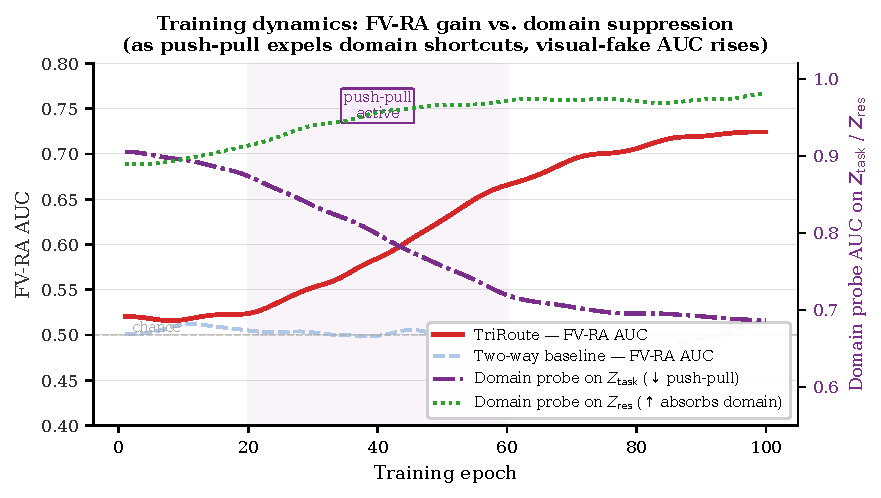
\includegraphics[width=0.82\linewidth]{training_dynamics.pdf}
    \caption{Training dynamics for \method. As domain push-pull suppresses shortcuts in $Z_{\mathrm{task}}$ (purple dash-dot, right axis), FV-RA AUC rises (red, left axis). $Z_{\mathrm{res}}$ absorbs expelled domain information (green dotted, right axis). The two-way baseline FV-RA stays near chance (blue dashed), isolating the factorization as the enabling condition.}
    \label{fig:training_dynamics}
\end{figure}

\subsection{Factor Geometry}

Figure~\ref{fig:tsne} visualises t-SNE embeddings of the two key factors. The residual factor $Z_{\mathrm{res}}$ forms tight, dataset-separated clusters, confirming it absorbs domain-specific nuisance. The task factor $Z_{\mathrm{task}}$ separates real from fake samples across all source domains without residual domain clustering, demonstrating that domain push-pull successfully prevents shortcut routing into the prediction head.

\subsection{Supplementary External Support on AVLips}

Table~\ref{tab:avlips} reports mean results over three seeds on AVLips, which provides only binary real/fake labels without modality-category annotations. The same ordering is preserved: two-way baseline $0.568$, three-way without push-pull $0.595$, \method\ $0.734$. This result is directionally consistent with the FakeAVCeleb benchmark, suggesting the routing-based improvement is not isolated to a single target dataset.

\begin{figure}[t]
    \centering
    
\includegraphics[width=0.97\linewidth]{tsne.pdf}
    \caption{t-SNE embeddings from a representative \method\ checkpoint. \textbf{Left}: $Z_{\mathrm{res}}$ forms tight dataset-specific clusters (colors), confirming it absorbs domain nuisance. \textbf{Right}: $Z_{\mathrm{task}}$ separates real (blue circles) from fake (red crosses) across all source domains without residual domain clustering.}
    \label{fig:tsne}
\end{figure}

\begin{table}[t]
    \centering
    \caption{AVLips cross-dataset AUC averaged over three independent seeds. Per-modality-category breakdown is unavailable; reported as supplementary directional evidence.}
    \label{tab:avlips}
    \small
    \begin{tabular}{lc}
        \toprule
        Method & Full AUC on AVLips \\
        \midrule
        Two-way baseline &  $0.5677$ \\
        Three-way, no domain push-pull &  $0.5954$ \\
        \method\ (ours) & $\mathbf{0.7340}$ \\
        \bottomrule
    \end{tabular}
\end{table}

\section{Limitations and Broader Impact}

\paragraph{Limitations.}
\method\ relies on speech-related evidence and may be less effective on deepfakes with minimal speaking motion, absent audio, or intentional desynchronization. The factorization introduces additional optimization complexity and requires reliable domain identifiers during training. The speaker-group pseudo-label is an extremely coarse domain proxy, yet the factorization substantially improves FV-RA, with the UDA setting contributing only modest additional gain ($+0.018$). Whether stronger or multi-source domain contrast yields further improvements remains open.

\paragraph{Broader impact.}
Cross-domain deepfake detection supports content authentication, media forensics, and platform integrity. Any detector can be misused for surveillance or overconfident moderation; we therefore recommend reporting calibration, failure modes, and domain-shift sensitivity alongside model releases, and releasing models with clear usage restrictions and dataset documentation.

\section{Conclusion}

We proposed \method, a three-way factorized audio-visual deepfake detector that separates shared content, modality-unique manipulation evidence, and residual domain-sensitive signal, restricting the prediction head to the first two components. On the AV1M$\rightarrow$FAVC cross-domain benchmark, \method\ substantially improves FV-RA AUC from $0.523$ to $0.659$ (no-target-data) and $0.677$ (UDA), while domain adversarial pressure on a two-way representation degrades FV-RA to $0.441$. Three-way factorization without domain supervision already reaches $0.626$, establishing structural separation as the primary driver. The small gap between label settings ($+0.018$) confirms that representation structure matters more than domain-label fidelity. Subspace probes identify the visual-unique channel as the strongest OOD carrier; head ablation and input perturbation both demonstrate concentrated routing dependence on that channel. Together, these analyses establish a routing-based explanation of the cross-domain gain.

\bibliographystyle{plainnat}
\bibliography{references}

\newpage
\input{checklist}

\end{document}
